\documentclass[]{article}
\usepackage{framed}
\usepackage{amsmath}
\usepackage{amssymb}
\usepackage{multicol}
\usepackage{graphicx}
%opening

\begin{document}

%---------------------------------------%
\section{Question 5 (Sample Variant 2)[25 marks]}

\begin{itemize}
%----------------------------------------------------- %
\item[(a)] \textbf{\textit{Binary Channels (5 Marks)}}\\

Consider the binary channel in the figure below.
\begin{figure}[h!]
\centering
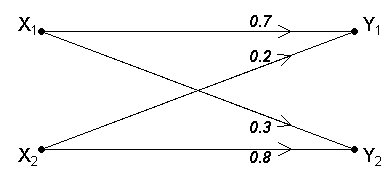
\includegraphics[width=0.7\linewidth]{./10Bnet3}
\caption{}
\label{fig:10Bnet3}
\end{figure}

\begin{itemize}
\item[(i)] (1 Marks) Determine the channel matrix of the channel
\item[(ii)] (2 Marks)  Find P($Y_1$) and P($Y_2$) when P($X_1$) = 0.7 and P($X_2$) = 0.3.
\item[(iii)] (2 Marks)  Find the joint probabilities P($X_1$, $Y_1$) and P($X_2$,$Y_2$).
\end{itemize}

%----------------------------------------------------- %
\item[(b)] \textbf{\textit{Huffman Coding (10 Marks)}}\\
A discrete memoryless source $X$ has five symbols $\{x_1,x_2,x_3,x_4,x_5\}$ with probabilities $P(x_1) = 0.45$ , $P(x_2) = 0.20$, $P(x_3) = 0.16$, $P(x_4) = 0.14$ and $P(x_5) = 0.05$.

\begin{itemize}
\item[(i)] (5 Marks) Construct a Huffman code for X.
\item[(ii)] (4 Marks) Calculate the efficiency of the code.
\item[(iii)] (1 marks) Calculate the redundancy of the code.
\end{itemize}

%----------------------------------------------------- %
\item(c) \item[(b)] \textbf{\textit{Shannon Coding (6 Marks)}}\\
A discrete memoryless source X has five symbols $\{x_1; x_2; x_3; x_4; x_5\}$ with prob-
abilities P(x1) = 0:40 , P(x2) = 0:25, P(x3) = 0:15, P(x4) = 0:12 and
P(x5) = 0:08.
\begin{itemize}
\item(i) (4 marks) Construct a Shanno code for $X$.
\item(ii) (2 marks) Calculate the entropy of the code.
%\item(iii) (2 marks) Calculate the redundancy of the code.
\end{itemize}


\item[(d)] \textbf{\textit{Communication Channels (4 Marks)}}\\
The input source to a noisy communication channel is a random variable X over the
four symbols $\{a, b, c, d\}$. The output from this channel is a random variable Y over these same
four symbols. \\
\noindent 
The joint distribution of these two random variables is as follows:\\ 
\begin{center}
\begin{tabular}{|c|c|c|c|c|}
\hline
y=a & 0.125	&	0.03125	&	0	&	0.015625	\\ \hline
y=b & 0	&	0.1875	&	0.125	&	0	\\ \hline
y=c & 0	&	0.015625	&	0.1875	&	0	\\ \hline
y=d & 0.0625	&	0	&	0	&	0.25	\\ \hline
\end{tabular}
\end{center}

\begin{itemize}
\item[(i)] (2 Marks) Write down the marginal distribution for $X$ and compute the marginal entropy $H(X)$.
\item[(ii)] (2 Marks) Write down the marginal distribution for $Y$ and compute the marginal entropy $H(Y )$.
\end{itemize}
\end{itemize}
\end{document}
